\chapter{Établir une connexion pair à pair}

\section{Avec WebRTC}

L'utilisation de WebRTC\footnote{Web Real-Time Communication} est l'une des solutions possibles pour mettre en place une communication textuelle en temps réel entre deux clients dans un réseau pair à pair.
Pour établir cette connexion, les étapes suivantes peuvent être suivies :

\paragraph{Initialisation d'une pair et récupération de son UUID}

Chaque client doit être initialisé en tant que pair et se voit attribuer un UUID\footnote{Universally Unique Identifier}. Cet identifiant est utilisé pour l'identifier et permettre à d'autres de s'y'connecter.

\paragraph{Partage des UUID entre les deux pairs}

Une fois que chaque noeuds a obtenu son UUID, ces identifiants doivent être partagés entre les deux clients afin qu'ils puissent s'identifier mutuellement lors de l'établissement de la connexion. 
Cela peut être réalisé par l'intermédiaire d'un serveur de signalisation ou d'un canal de communication préalablement établi, tel qu'un serveur centralisé ou un autre moyen de communication sécurisé.

\paragraph{Création d'une connexion entre les deux pairs}

Une fois que chaque pair dispose de l'UUID de l'autre, ils peuvent utiliser ce dernier pour établir une connexion directe entre eux en utilisant le protocole WebRTC. Ce dernier permet aux clients d'établir des connexions directes,
contournant ainsi les NAT et réduisant la latence. Le tou grace à l'utilisation de protocoles de traversée NAT (NAT traversal protocol) ou les techniques de trous de poinçonnage (hole punching) pour contourner les limitations des NAT.

\begin{figure}[h]
    \centering
    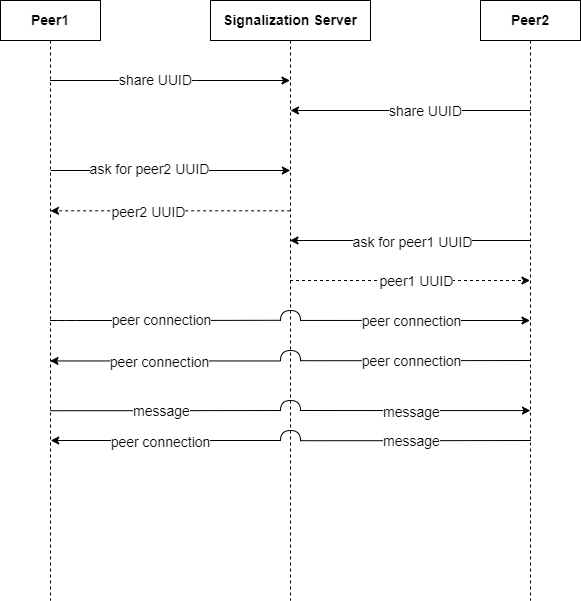
\includegraphics[width=0.9\textwidth]{assets/webrtc.png}
    \caption{Schéma de connection avec WebRTC}
    \label{fig:webrtc}
\end{figure}

\newpage

\paragraph{}
Pour pouvoir fonctionner, WebRTC utilise le protocole ICE (Interactive Connectivity Establishment) qui permet de contourner les limitations des NAT et de trouver le chemin le plus efficace pour établir une connexion entre les deux pairs. 
Ce protocole utilise les techniques de "trou de poinçonnage" (hole punching) pour contourner les limitations des NAT. Et ce grace grace à un serveur STUN qui permet de récupérer l'adresse IP publique et le port du client.
Une fois que les deux pairs ont récupéré leurs adresses publiques, ils peuvent s'échanger leurs adresses et ports privés. Cela permet aux deux pairs de s'envoyer des paquets directement sans passer par le serveur STUN. 

\paragraph{}
Par défaut, la librairie WebRTC du navigateur utilise un serveur STUN de Google\footnote{stun.l.google.com:19302} pour récupérer l'adresse IP publique et le port du client. Cependant, il est possible de configurer un serveur STUN personnalisé pour effectuer cette tâche.
Chose que j'ai faite en utilisant le serveur STUN fourni par la librairie coturn\footnote{coturn.net}. Coturn est un serveur TURN et STUN open source qui permet de configurer un serveur STUN personnalisé. Une fois le serveur configuré, il suffit de le spécifier dans 
la configuration de la librairie WebRTC du navigateur.

\paragraph{}
Afin de vérifier le bon fonctionnement du serveur STUN, j'ai utilisé l'outil Trickle ICE\footnote{https://webrtc.github.io/samples/src/content/peerconnection/trickle-ice/} qui permet de récupérer les adresses IP et ports utilisés par la librairie WebRTC du navigateur.
En utilisant cet outil, j'ai pu vérifier que les adresses IP et ports récupérés sont bien ceux du serveur STUN configuré. 


\newpage
\section{Avec libp2p}

\paragraph{}
Libp2p\footnote{https://libp2p.io/}, (pour "bibliothèque peer-to-peer") est un cadre de mise en réseau peer-to-peer (P2P) qui permet le développement des applications P2P. Il se compose d'une collection de protocoles, de spécifications et bibliothèques qui 
facilitent la communication P2P entre les participants au réseau, appelées "pairs". Libp2p fournit une interface de programmation d'application (API) pour les applications P2P, ainsi que des implémentations de ces protocoles.

\paragraph{}
Dans un premier temps développé pour le projet IPFS\footnote{InterPlanetary File System}, libp2p, a au fil du temps été mit à jour et amélioré pour être utilisé dans d'autres projets. Il est aujourd'hui réputé pour sa modularité, sa sécurité et sa résilience. C'est un outil
puissant pour effectuer des tâches comme le "trou de poinçonnage" (hole punching), la distribution et la diffusion de contenu, la découverte de pairs, la communication sécurisée, etc. 

\paragraph{}
Libp2p est un framework qui permet de créer des applications pair à pair. Il est composé de plusieurs modules qui peuvent être utilisés indépendamment les uns des autres. Il est également possible d'ajouter des modules personnalisés
pour répondre à des besoins spécifiques. 


Pour établir une connexion pair à pair avec libp2p, les étapes suivantes peuvent être suivies :
\paragraph{Initialisation des nœuds}
Chaque nœud initialise sa propre instance de Libp2p en configurant les fonctionnalités et les protocoles souhaités.

\paragraph{Découverte des pairs}
Les nœuds utilisent des mécanismes de découverte pour trouver d'autres pairs disponibles dans le réseau. Cela peut se faire en utilisant des serveurs de rendez-vous, des protocoles de découverte basés sur DHT (Distributed Hash Table), etc.

\paragraph{Échange des adresses multiadresses}
Une fois que les nœuds ont découvert d'autres pairs, ils s'échangent mutuellement leurs adresses multiadresses. Une adresse multiadresse est une adresse qui encapsule différentes informations, telles que l'adresse IP, le port, les protocoles pris en charge, etc.

\paragraph{Négociation des protocoles}
Les nœuds négocient les protocoles qu'ils souhaitent utiliser pour la communication. Cela peut inclure des protocoles spécifiques à une application ou des protocoles de base fournis par Libp2p, tels que TCP\footnote{Transmission Control Protocol}, WebSockets, etc.

\paragraph{Établissement de la connexion}
Les nœuds utilisent les adresses multiadresses échangées précédemment pour établir une connexion directe. Cela peut impliquer l'établissement d'une connexion TCP, l'établissement d'une connexion WebSockets, ou d'autres mécanismes de transport pris en charge.

\paragraph{Handshake sécurisé}  
Une fois la connexion établie, les nœuds peuvent effectuer un handshake sécurisé pour s'authentifier mutuellement et échanger des clés de chiffrement. Cela peut se faire en utilisant des protocoles de chiffrement tels que TLS\footnote{Transport Layer Security}.

\paragraph{Communication }
Une fois que la connexion est établie et sécurisée, les nœuds peuvent commencer à échanger des données selon les protocoles applicatifs spécifiques. Cela peut impliquer l'utilisation de protocoles de haut niveau pour la transmission des messages, le partage de fichiers, etc.


\section{Le cas de WebSockets}

\paragraph{}
Les WebSockets sont un protocole de communication bidirectionnel qui permet d'établir une connexion persistante entre un client et un serveur. Contrairement au protocole HTTP\footnote{Hypertext Transfer Protocol}, qui est un protocole de communication unidirectionnel, 
les WebSockets permettent aux clients et aux serveurs de s'envoyer des données à tout moment, sans avoir à attendre une requête du client. 

\paragraph{}
Les WebSockets sont souvent utilisés pour les applications qui nécessitent une communication bidirectionnelle en temps réel, telles que les applications de chat, les jeux en ligne, etc. Ils sont également utilisés pour les applications qui nécessitent une communication
persistante entre le client et le serveur, telles que les applications de suivi en temps réel, les applications de surveillance, etc. 

\paragraph{}
Les WebSockets sont un protocole de communication de haut niveau qui s'appuie sur le protocole TCP pour établir une connexion. Ils sont souvent utilisés avec des protocoles de haut niveau tels que HTTP, TLS, etc. pour établir une connexion sécurisée.

\paragraph{}
Nous avons ici pensé à utiliser les WebSockets pour établir une connexion entre les deux pairs. En effet, les sockets se divisent en deux parties, un serveur et un client. Le serveur est le programme qui attend les connexions des clients et le client est le programme qui se connecte au serveur.
Dans notre cas, chaque pair peut être considéré comme un serveur et un client. En effet, chaque pair doit être capable d'accepter les connexions des autres pairs et de se connecter aux autres pairs. Nous avons donc tenté de créer un serveur WebSocket dans chaque pair et de connecter les deux serveurs entre eux.

\paragraph{}
Cependant, nous avons rencontré un problème lors de la mise en place de cette solution. En effet, comme évoqué plus tôt, le NAT empêche toute communication entrante vers un client. Cela signifie que le serveur WebSocket ne peut pas recevoir de connexion entrante d'un autre pair.
Pour contourner ce problème, nous avons pensé à mettre ne place un tiers serveur qui permettrait de faire le lien entre les deux pairs. Chaque client via un serveur STUN pourrait récupérer son adresse IP publique et son port et les envoyer au serveur afin que par la suite, chaque 
client qui souhaite établir une connexion n'ai qu'à récupérer l'adresse IP publique et le port de l'autre client et se connecter à ce dernier.
